\let\negmedspace\undefined
\let\negthickspace\undefined
\documentclass[journal]{IEEEtran}
\usepackage[a5paper, margin=10mm, onecolumn]{geometry}
%\usepackage{lmodern} % Ensure lmodern is loaded for pdflatex
\usepackage{tfrupee} % Include tfrupee package

\setlength{\headheight}{1cm} % Set the height of the header box
\setlength{\headsep}{0mm}     % Set the distance between the header box and the top of the text

\usepackage{gvv-book}
\usepackage{gvv}
\usepackage{cite}
\usepackage{amsmath,amssymb,amsfonts,amsthm}
\usepackage{algorithmic}
\usepackage{graphicx}
\usepackage{textcomp}
\usepackage{xcolor}
\usepackage{txfonts}
\usepackage{listings}
\usepackage{enumitem}
\usepackage{mathtools}
\usepackage{gensymb}
\usepackage{comment}
\usepackage[breaklinks=true]{hyperref}
\usepackage{tkz-euclide} 
\usepackage{listings}
% \usepackage{gvv}                                        
\def\inputGnumericTable{}                                 
\usepackage[latin1]{inputenc}                                
\usepackage{color}                                            
\usepackage{array}                                            
\usepackage{longtable}                                       
\usepackage{calc}                                             
\usepackage{multirow}                                         
\usepackage{hhline}                                           
\usepackage{ifthen}                                           
\usepackage{lscape}
\begin{document}

\bibliographystyle{IEEEtran}

\title{10.7.72}
\author{EE25BTECH11023 - Venkata Sai}
% \maketitle
% \newpage
% \bigskip
\maketitle 
\renewcommand{\thefigure}{\theenumi}
\renewcommand{\thetable}{\theenumi}
\setlength{\intextsep}{10pt} % Space between text and floats

\numberwithin{align}{enumi}
\numberwithin{figure}{enumi}
\renewcommand{\thetable}{\theenumi}

\textbf{Question:}  \\
The chords of contact of the pair of tangents drawn from each point on the line
$2x + y = 4$ to $x^2 + y^2 = 1 $ pass through the point $\dots$\\
\textbf{Solution:}  \\
The general equation of conic
\begin{align}
    \vec{x}^\top\vec{V}\vec{x} + 2\vec{u}^\top\vec{x} + f = 0
\end{align}
The chord of contact of tangents from an external point $\vec{q}$ is given by
\begin{align}
 \brak{\vec{V}\vec{q}+\vec{u}}^\top\vec{x}+\vec{u}^\top\vec{q}+f=0
\end{align}
Given circle in matrix form
\begin{align}
x^2 + y^2 &= 1  \\
x^2 + y^2 - &1=0 \\
\vec{x}^\top\myvec{1 &0 \\0 &1}\vec{x}&-1=0
\end{align}
where
\begin{align}
\vec{V}=\myvec{1&0\\0&1}=\vec{I},\vec{u}=\vec{0},f=-1
\end{align}
Given line 
\begin{align}
2x + y = 4 \\ 
\myvec{2&1}\vec{x}=4
\end{align}
As $\vec{q}$ satisfies \brak{8}
\begin{align}
   \myvec{2&1}\vec{q}=4 
\end{align}
From \brak{2} and \brak{6}
\begin{align}
  \brak{\vec{I}\vec{q}+\vec{0}}^\top\vec{x}&+\vec{0}^\top\vec{q}-1=0 \\
  \brak{\vec{I}\vec{q}}^\top\vec{x}&-1=0\\
  \vec{q}^\top\vec{x}&-1=0\\
  \vec{q}^\top\vec{x}=1&\implies
  \vec{x}^\top\vec{q}=1 
  \end{align}
From \brak{9} and \brak{13} 
\begin{align}
    \vec{x}^\top&=k\myvec{2&1}\\
    \brak{k\myvec{2&1}}^\top\vec{q}=1&\implies
    k\myvec{2&1}^\top\vec{q}=1\\
    k\brak{4}=1 &\implies k=\frac{1}{4}\\
    \vec{x}^\top=\frac{1}{4}\myvec{2&1} &\implies \vec{x}^\top=\myvec{\frac{1}{2}&\frac{1}{4}}\\
    \vec{x}&=\myvec{\frac{1}{2}\\\frac{1}{4}}
\end{align}
Hence the chords of contact pass through the point  $\myvec{\frac{1}{2}\\\frac{1}{4}}$
\begin{figure}[h!]
   \centering
   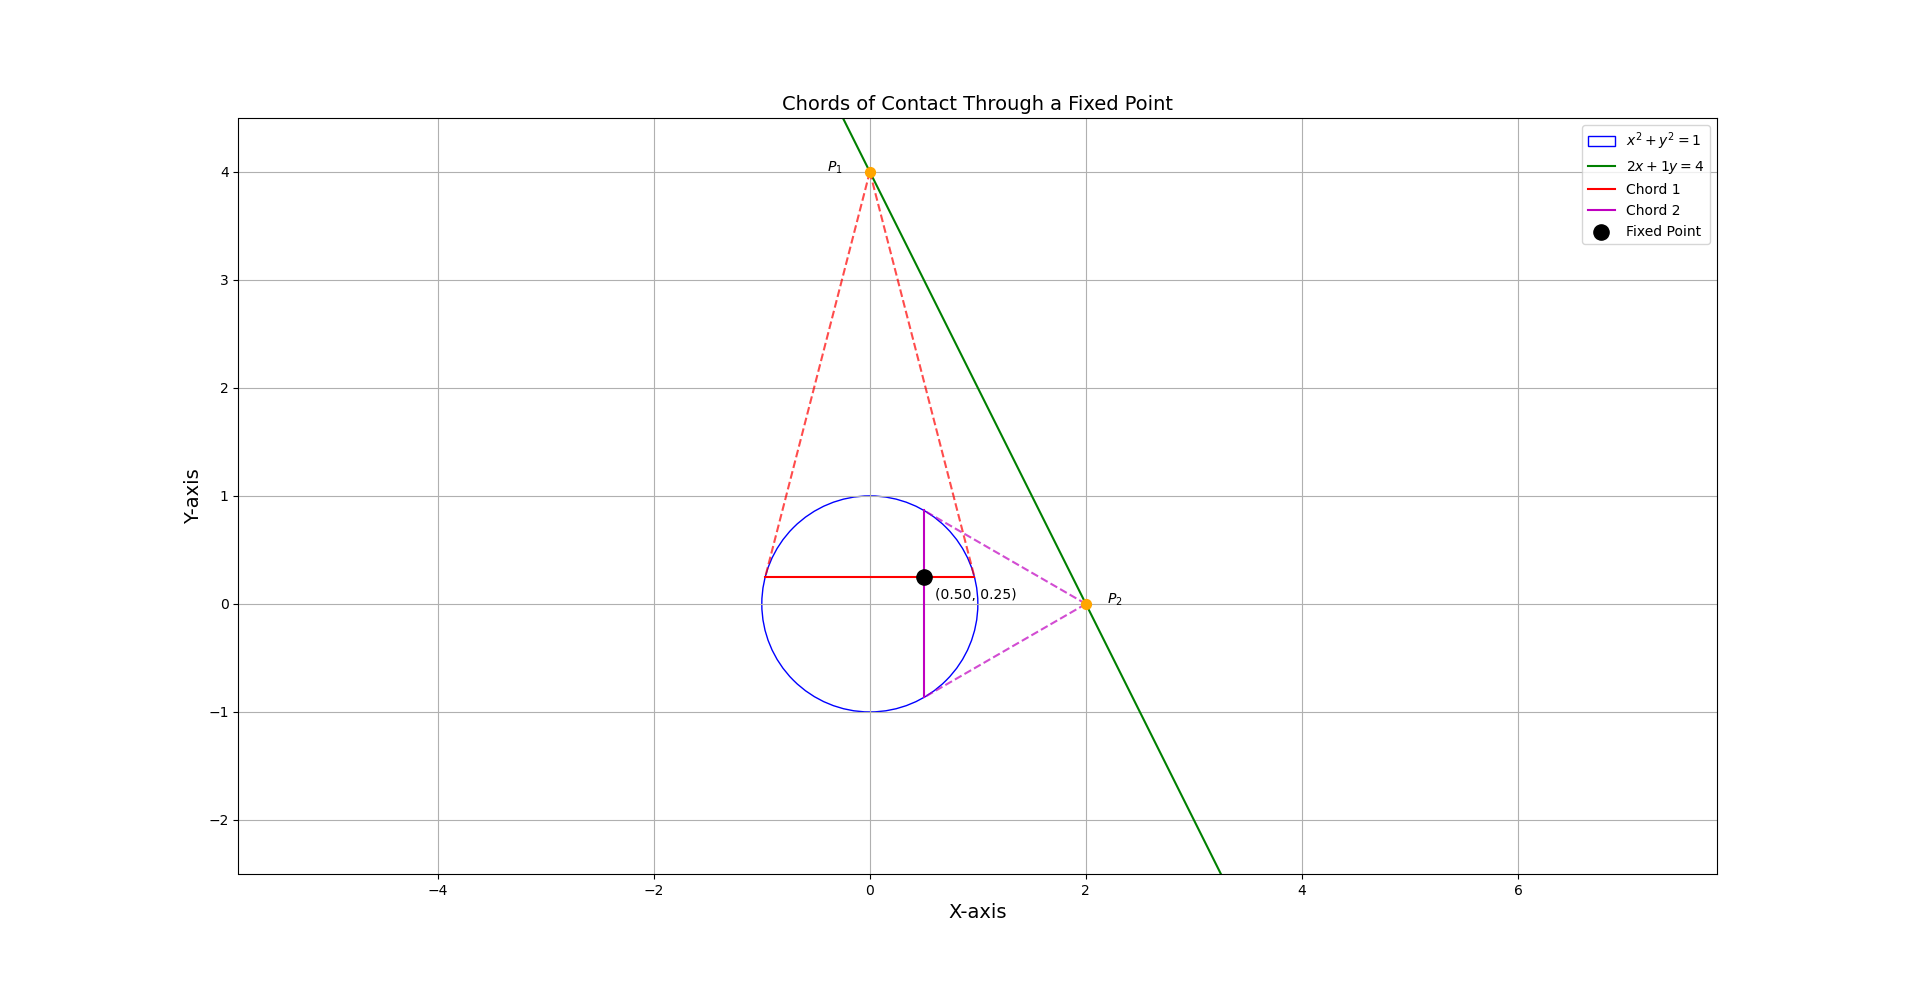
\includegraphics[width=0.9\columnwidth]{figs/fig1.png}
	\caption{}
   \label{}
\end{figure}
\end{document}  
